% =========================================================
% Main File
% =========================================================

% Bem vindo(a) a este template destinado a trabalhos
% acadêmicos da disciplina de ASD.
% A distribuição deste template é encorajada.
%
% Autor: Leonardo A. Antunes
% Professor: Geraldo C. Brito Jr.
%
% Disponível no Github:
% https://github.com/AntunesLeonardo/LaTeX_Template/tree/master/ASD_Template
% Disponível no Overleaf:
% https://www.overleaf.com/read/vsfrktpqnbzh

\documentclass{ASD_LaTeX}

\author{Autor Autor Autor}
\authorabbreviate{A. A. Autor}
\authoremail{fulano@somewhere.com}

\title{Título}
\edition{2\textsuperscript{nd} Sysdin}
\location{Iguassu Falls, Paraná - Brazil}
\city{Foz do Iguaçu, PR, Brazil}
\address{Av. Tancredo Neves, 6731 - Jardim Itaipu, 85.867-900, Paraná, PR, Brasil}
\date{January 1\textsuperscript{ST}}
\theyear{2022}

\institution{Unioeste}
\graduation{Engenharia Elétrica}
\professor{G.C. Brito Jr.}

% Comente os elementos não desejados no seu projeto:

\begin{document}
    %% =========================================================
% Contents File
% =========================================================
    % =========================================================
% Exemples File
% =========================================================

\abstractAndKeyWords{
    Não devem ser utilizados títulos genéricos como”1o Artigo de Análise de Sistemas Dinâmicos”, o título do artigo deverá refletir exatamente o que foi feito.
    A seção de resumo deverá conter de 150 a 250 palavras (use a ferramenta “Contagem de Palavras” no menu “Revisão”) descrevendo a motivação do artigo, o que foi realizado, como foi realizado, além dos principais resultados obtidos.
    O artigo deverá ser enviado à coordenação do evento em formato pdf, juntamente com todo o material utilizado para fazê-lo (versão em formato Word, scripts Matlab, manuscritos para dedução das equações governantes do sistema etc.).
    O número máximo de páginas do artigo é 12, as páginas excedentes serão penalizadas com 5 pontos na nota.
    Portanto, devem ser evitadas repetições desnecessárias.
    As fontes ou a formatação deste documento não devem ser mudadas, devendo ser preenchidos todos os campos, inclusive cabeçalhos e rodapés.
    Alterações serão penalizadas, em caso de dúvidas a coordenação do evento deve ser contatada.
    As palavras-chave devem refletir o sistema dinâmico analisado e as ferramentas utilizadas (Série de Fourier Discreta, Transformada de Fourier Discreta, Função de Resposta ao Impulso, Convolução, Transformada de Laplace, Função de Resposta em Frequência, Matriz de Funções de Transferência, Equação de Estado etc.) para fazê-lo.
    As referências devem ser citadas por nome e (ano), as referências devem ser listadas ao final do artigo em uma seção apropriada, em ordem alfabética.
    Deverá ser utilizado preferencialmente o gerenciador de fontes bibliográficas do Word, ferramenta útil em outros trabalhos como o Trabalho de Conclusão de Curso (TCC).
    }{1ª Palavra-chave, 2ª Palavra-chave, ...,5ª Palavra-chave (até 5 palavras-chave)}

\section{Introdução}

Nesta seção é esperada uma descrição \underline{detalhada} do sistema que será analisado, incluindo figuras e tabelas trazendo informações sobre os principais parâmetros deste sistema.
Esta seção também deverá descrever as justificativas e a motivação da análise, as ferramentas utilizadas, as condições de contorno do estudo e outros informações pertinentes e relevantes.
O artigo deverá permitir que que outros engenheiros possam reproduzir os estudos e análises apresentados.

As figuras, tabelas e equações devem ser numeradas na forma mostrada neste documento, devendo ser citadas pelos números e descritas de forma adequada \underline{antes} de aparecerem no texto.
Nunca deixe uma figura, tabela ou equação dispersa no artigo.
Por exemplo, a Figura \ref{fig:tras-trifasico} mostra a vista do sistema dinâmico analisado neste artigo, um transformador de potência trifásico 500kV/760kV, com 1000 MVA de capacidade e isolado com óleo mineral e hexafluoreto de enxofre (SF\textsubscript{6}).
Os parâmetros principais deste transformador são mostrados na Tabela \ref{tab:dados}.
Deverá ser utilizada preferencialmente a ferramenta \quo{Referência Cruzada}, no menu \quo{Referências}; ela é uma ferramenta muito útil para engenheiros, na redação de artigos ou relatórios técnicos.

\begin{figure}[htb]
    \centering
    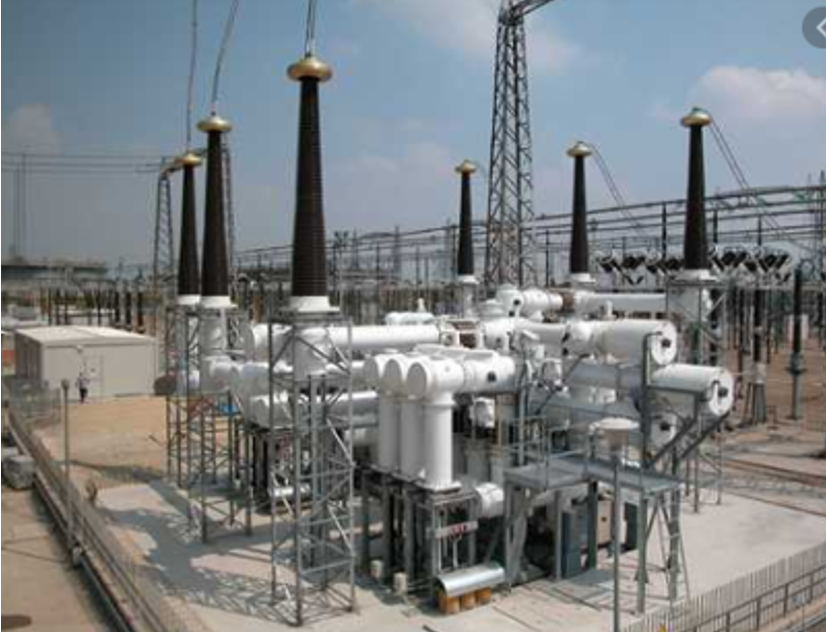
\includegraphics[width=0.6\textwidth]{images/transformador_trifasico.png}
    \caption{Vista de um transformador de potência trifásico 500 kV/760 kV de 1000 MVA de capacidade.}
    \label{fig:tras-trifasico}
\end{figure}

Observe que eventuais textos nas figuras deverão ser legíveis, usando um tamanho de fonte compatível com o tamanho utilizado nas legendas (tamanho 10).
As legendas das figuras e tabelas devem ser capazes de permitir ao leitor extrair as principais informações sem que ele tenha que recorrer ao texto para entendê-las ou contextualizá-las.
Exemplo de citação \cite{lathi2006sinais}.

\begin{table}[htb]
    \footnotesize
    \centering
    \caption{Parâmetros do transformador de potência trifásico analisado}
    \label{tab:dados}
    \begin{tabular}{ccc}
        \hline
        \textbf{Parâmetro}    & \textbf{Unidade} & \textbf{Valor} \\ \hline
        Tensões primárias     & KV               & 500            \\
        Tensões no secundário & KV               & 760            \\
        Capacidade            & MVA              & 1000           \\
        Isolação              & --               & Óleo / SF6     \\ \hline
    \end{tabular}
\end{table}

\section{Fundamentação teórica e metodologia}

Esta seção contém uma descrição resumida da \quo{Fundamentação Teórica} e da \quo{Metodologia} utilizadas na elaboração deste artigo.

\subsection{Fundamentação Teórica}

Esta subseção deverá conter uma descrição resumida das ferramentas que foram utilizadas no artigo, como, por exemplo, das ferramentas de processamento de sinais (Série de Fourier Discreta, Transformada de Fourier Discreta, Transformada de Fourier de Curto Termo) e da modelagem matemática do sistema.
Nesta seção deverá aparecer as principais equações que governam o sistema estudado.
Por exemplo, a Equação (\ref{eq:vibracoes}) mostra as equações de movimento que descrevem as vibrações do núcleo do transformado em estudo:

\begin{equation}
    \label{eq:vibracoes}
    \begin{Bmatrix}
        f_1(t) \\ f_2(t)
        \end{Bmatrix}
        =
        \begin{bmatrix}
        m_n & 0 \\
        0 & m_n \\
        \end{bmatrix}
        \begin{Bmatrix}
        \ddot{z}_1(t) \\ \ddot{z}_2(t)
        \end{Bmatrix} 
        +
        \begin{bmatrix}
        c_{n1} & 0 \\
        0 & c_{n2} \\
        \end{bmatrix}
        \begin{Bmatrix}
        \dot{z}_1(t) \\ \dot{z}_2(t)
        \end{Bmatrix} 
        +
        \begin{bmatrix}
        k_{n1} & 0 \\
        0 & k_{n2} \\
        \end{bmatrix}
        \begin{Bmatrix}
        z_1(t) \\ z_2(t)
        \end{Bmatrix}
        \text{,}
\end{equation}

onde $f_i(t)$ são as forças eletromagnéticas de excitação nas direções $z_i (i=1,2)$.
Ainda nesta equação $m_n$ é a massa do núcleo, $c_{ni}$ são os coeficientes de amortecimento e $k_{ni}$ são os coeficientes de rigidez, nas direções $z_i$.

Deve-se observar que a Equação (\ref{eq:vibracoes}) foi apresentada ao leitor como se fosse parte do texto, após a equação há uma \quo{vírgula} e o texto que segue a ela está no mesmo parágrafo, iniciado propositalmente em letra minúscula para mostrar isso.

Esta subseção deverá conter uma \underline{descrição resumida} das ferramentas que foram utilizadas no artigo, como, por exemplo, das ferramentas de processamento de sinais (Série de Fourier Discreta, Transformada de Fourier Discreta, Transformada de Fourier de Curto Termo) e da modelagem matemática do sistema.

\subsection{Metodologia}

Nesta subseção deverá ser descrita a metodologia utilizada na análise do sistema dinâmico estudado, fornecendo ao leitor elementos e informações suficientes para julgar se o estudo é válido, reprodutível e aplicável em outros estudos.
Geralmente ela contém uma revisão da literatura, mostrando os resultados de colegas da área em estudos anteriores.
Neste tipo de artigo a revisão da literatura foi substituída pela subseção anterior (Fundamentação Teórica), mais indicada para artigos durante o curso de graduação.

A seção deverá apresentar o tipo de pesquisa realizada, os dados a serem obtidos, a forma de obtenção dos dados, o tratamento e análise dos dados (processamento de sinais), as aplicações e as limitações da pesquisa (pontos fortes e pontos fracos).
Também deverão ser descritas a metodologia utilizada nas simulações que serão apresentadas no artigo, além dos softwares e dos scripts utilizados para tais fins.
Esta subseção poderá ser subdividida caso seja necessário.

\section{Resultados Obtidos}

Nesta seção deverão ser apresentados os principais resultados obtidos na análise realizada.
Pela característica dos temas apresentados esta seção pode ser quase sempre dividida em duas subseções, como as descritas a seguir.

\subsection{Resultados relacionados ao processamento de sinais}

Esta subseção descreve os principais resultados obtidos relacionados à área de processamento de sinais.
O título deverá refletir o conteúdo apresentado. Se for necessário esta subseção poderá ser subdividida.

\subsection{Resultados relacionados à simulação de sistemas}

Esta subseção descreve os principais resultados obtidos relacionados à área de simulação de sistemas.
O título deverá refletir o conteúdo apresentado.
Se for necessário esta subseção poderá ser subdividida.

\section{Conclusões e Futuros Trabalhos}

Esta seção deverá descrever de forma resumida as principais conclusões e observações feitas no artigo.
Ela deve conter ainda as simplificações e limitações dos modelos, simulações e processamento de sinais, além de possíveis melhorias que poderão ser introduzidas em trabalhos futuros.

\biblio
    %\begin{appendices}
    \section{Teste de apêndice}
\end{appendices}
\end{document}